% Cluster analysis
\chapter{Cluster analysis} \label{s:ap:cs}

\newpage 

% Non-PCA
\section{Non-PCA} \label{s:ap:non-pca}

This section presents the cluster metric plots (Davies Bouldin, Calinski Harabasz, and Silhouette) for the models used in \cref{s:cs:right_config}. The key difference between the two experiments is that, in \cref{s:ap:non-pca}, the expression of the 3,500 genes is not reduced to the 5 Principal Components, as was done in \cref{s:cs:right_config}. The following plots show that the metrics perform worse across all three clustering scores compared to the cluster analysis with the data PCA-transformed.


\begin{figure}[!htb]    
    \centering
    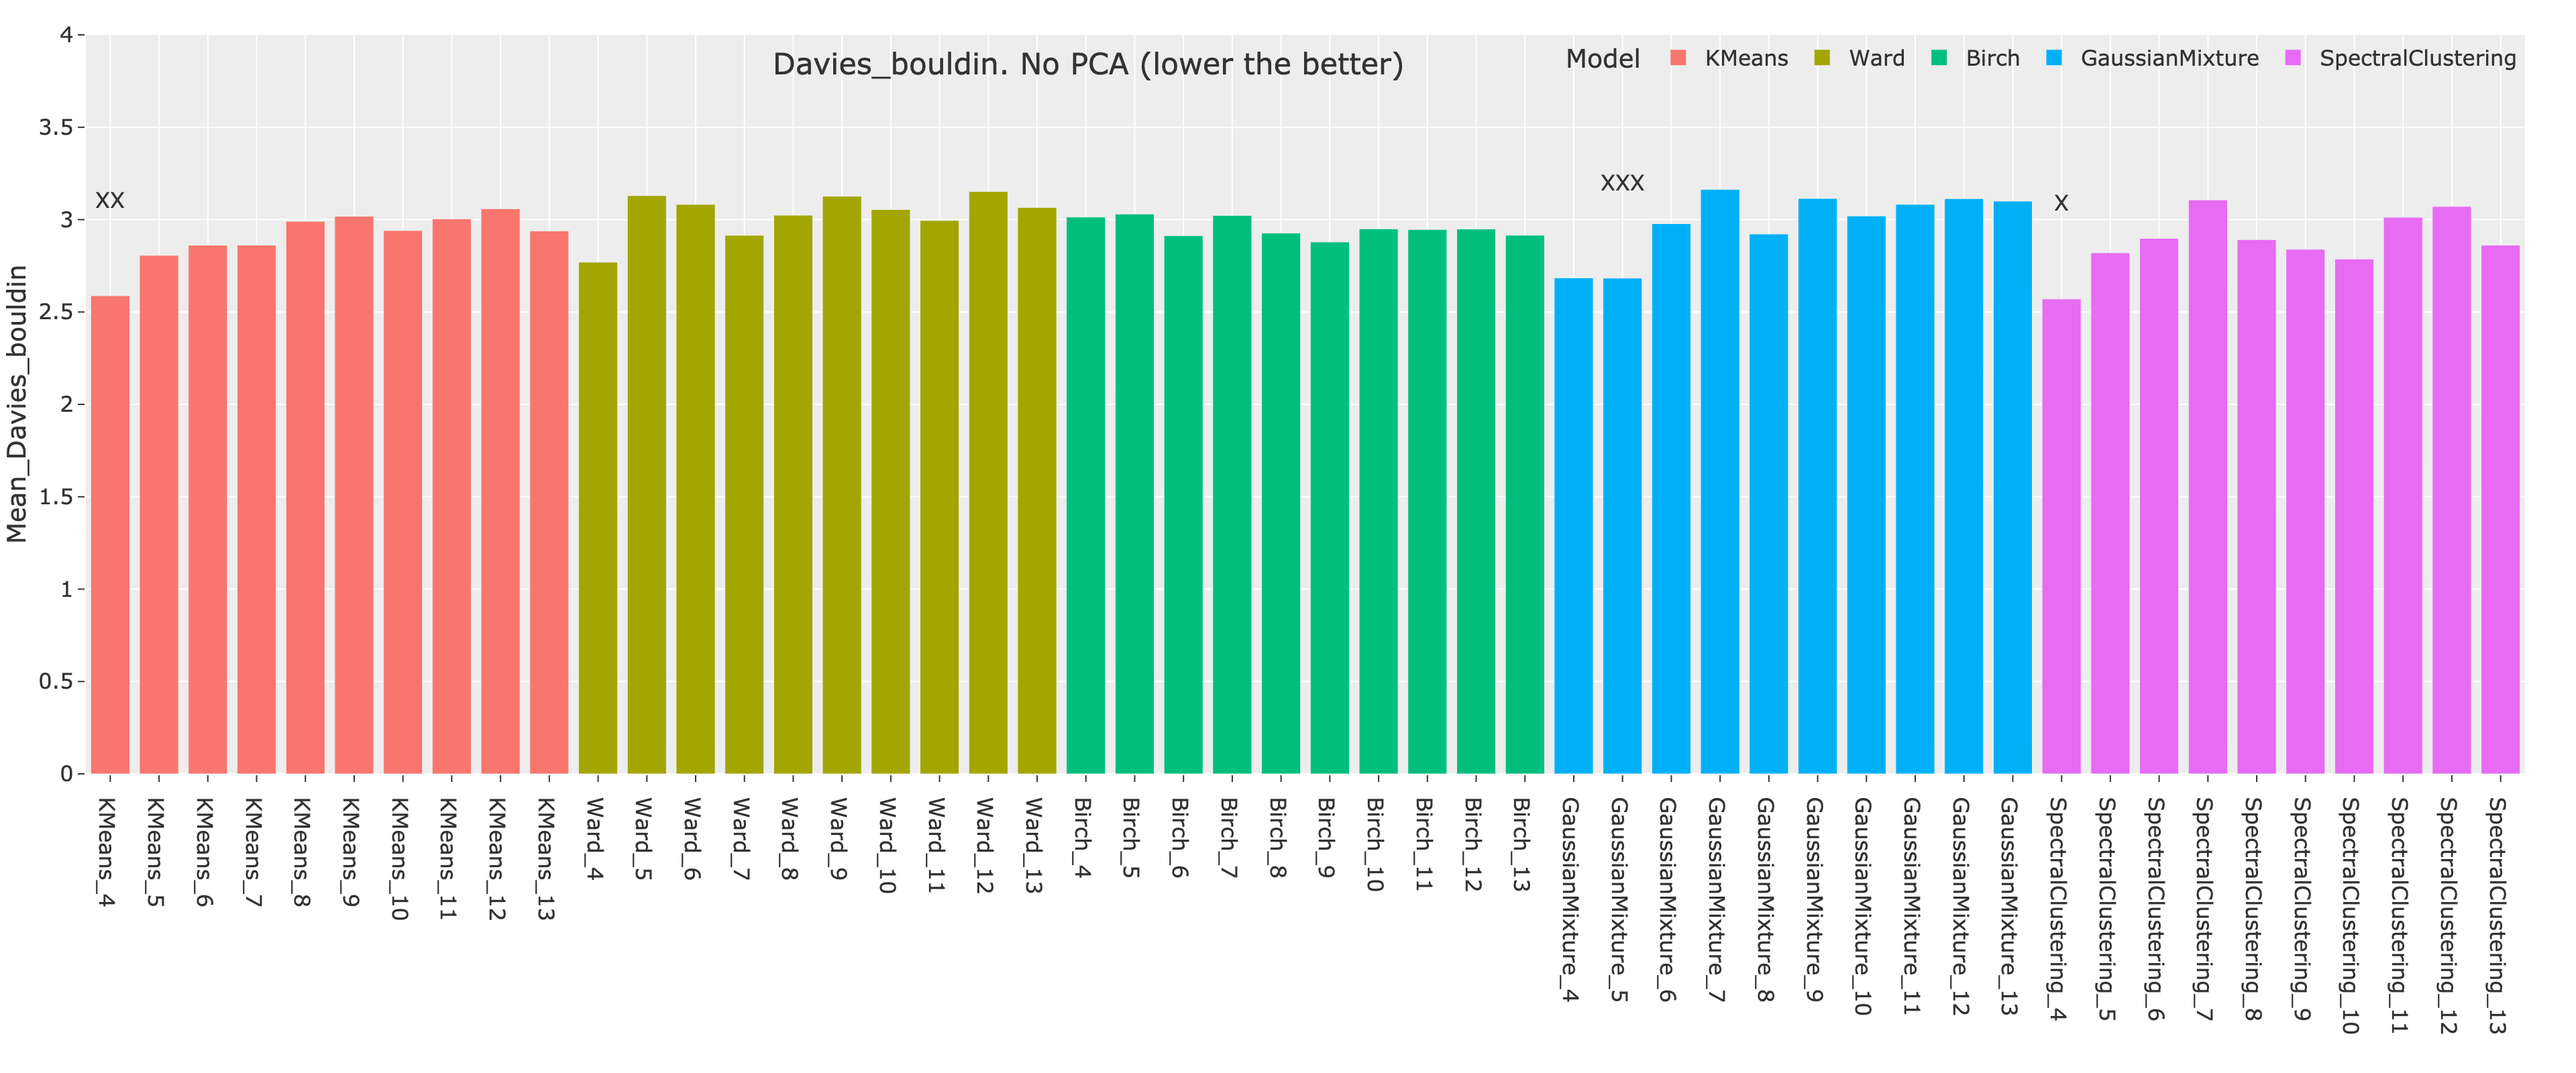
\includegraphics[width=1.0\textwidth,keepaspectratio]{Sections/ClusteringAnalysis/Resources/cs_top3/non_PCA_top3_Davies_bouldin.png}
    \caption[Non-PCA transformed data: Davies Bouldin]{The means of the cluster metrics introduced by Davies-Bouldin, as described in \cref{s:lit:clustering_metrics}. For each metric, the top 3 performing models are marked by "X". Gaussian Mixture Model is abbreviated as GM, and Spectral Clustering as SC. Spectral Clustering with K=4 and K-means with K=4 are the two best-performing models. The difference between this plot and the one in \cref{fig:cs:dav_boul} is that the gene expression data here is not PCA-transformed. Overall, the non-PCA experiments perform worse compared with the PCA-transformed data in Davies-Bouldin scores and the other two cluster metrics in \cref{fig:ap:non_pca_metrics}.}
    \label{fig:ap:non_pca_dav_boul}
\end{figure}



\begin{figure}[H]
    \centering
    \begin{subfigure}[!t]{1.0\textwidth}
        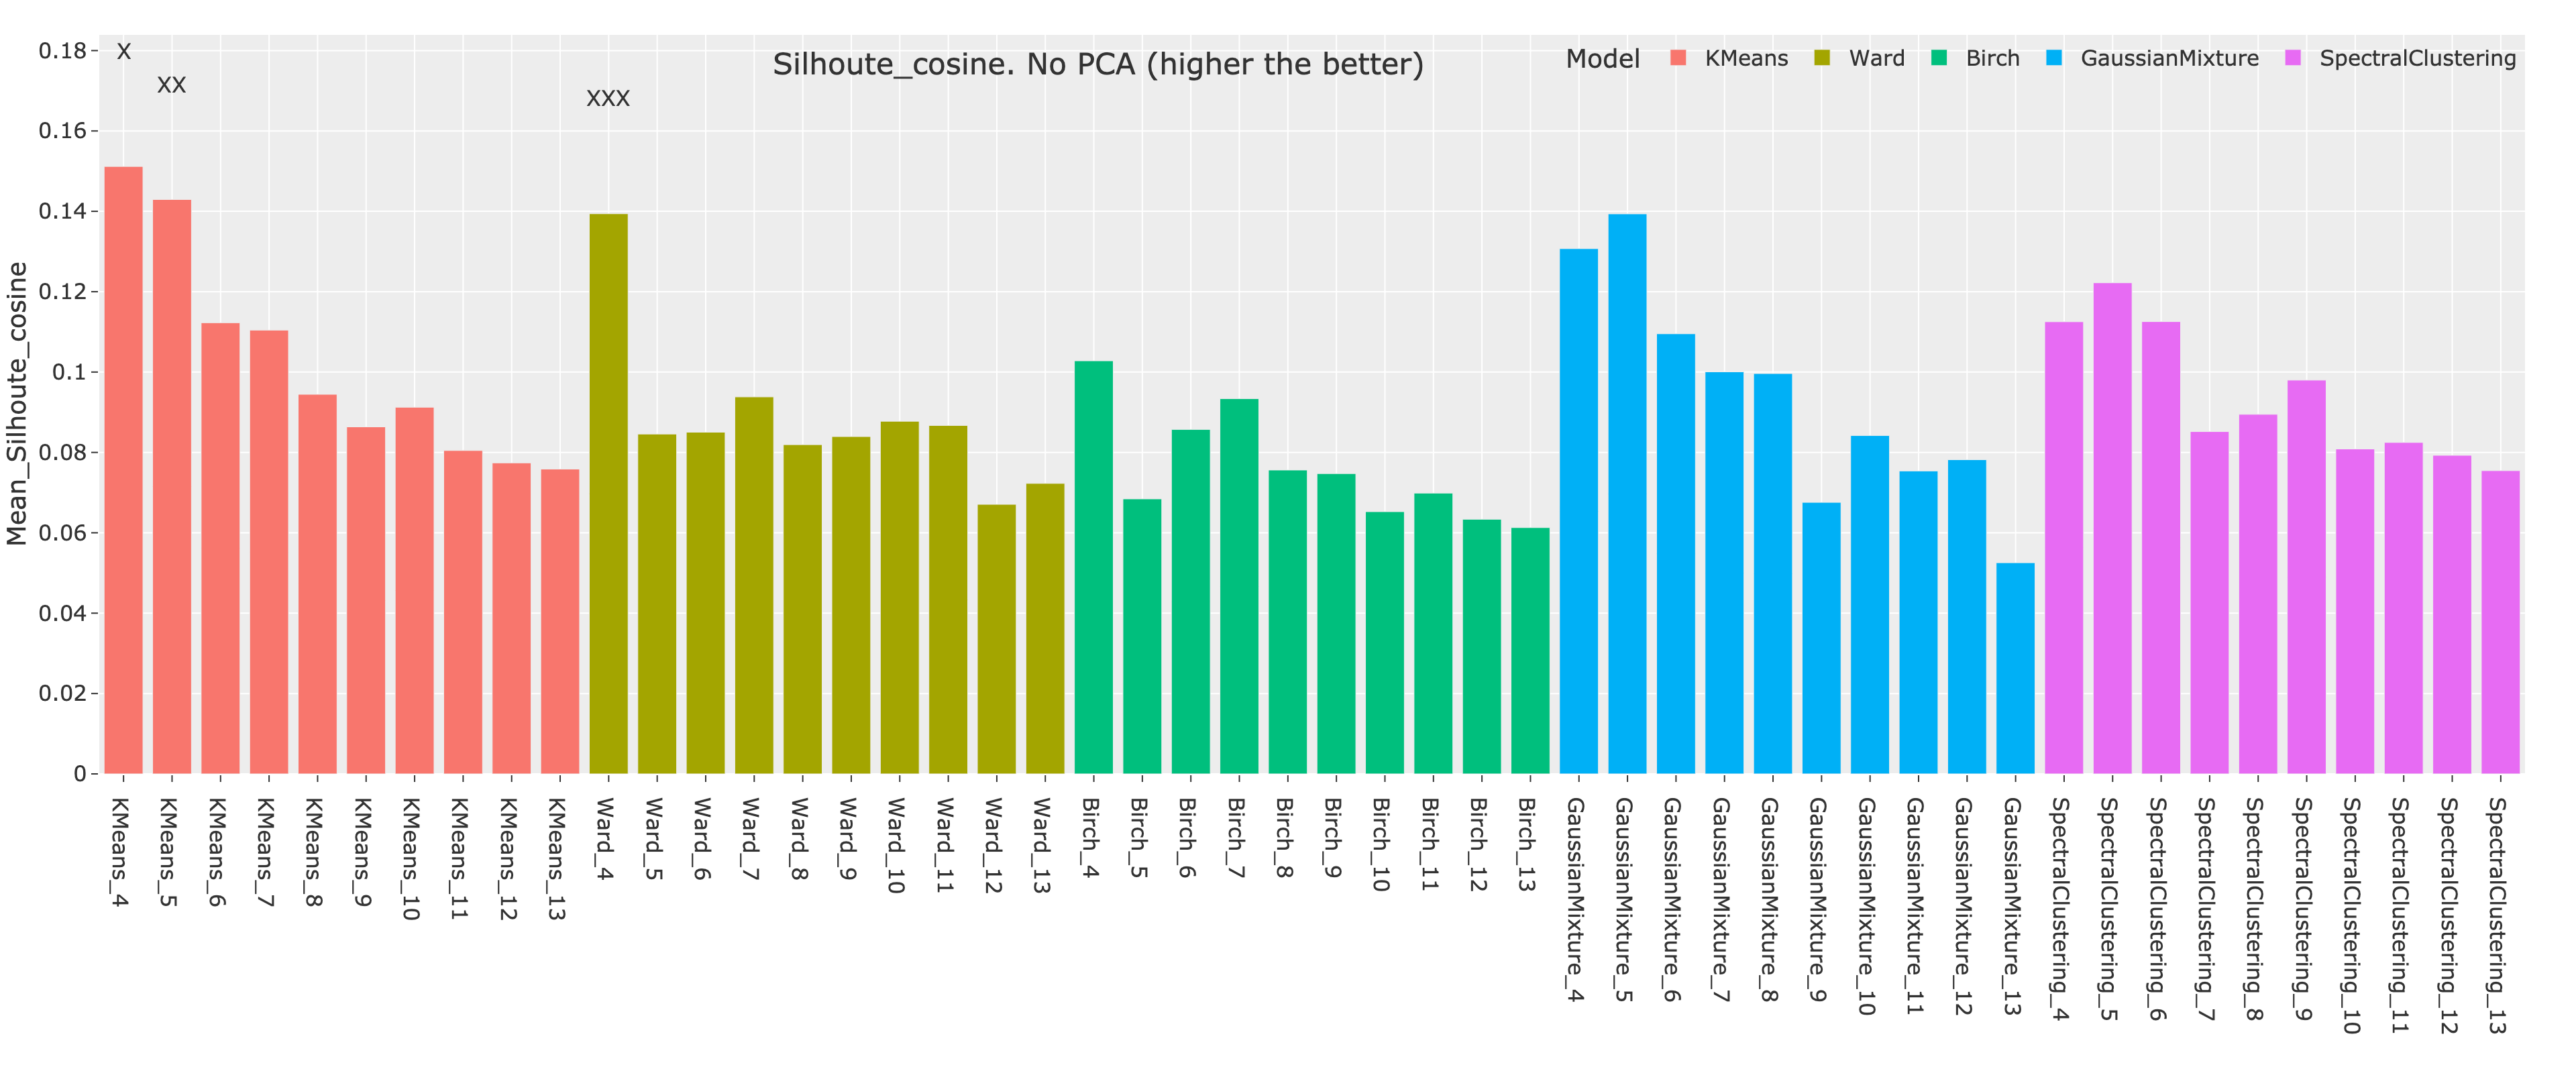
\includegraphics[width=\textwidth,keepaspectratio]{Sections/ClusteringAnalysis/Resources/cs_top3/non_PCA_top3_Silhoute_cosine.png}
        \caption{Silhouette using cosine distance}
        \label{fig:ap:cosine}
    \end{subfigure}
    \centering
    \begin{subfigure}[!t]{1.0\textwidth}
        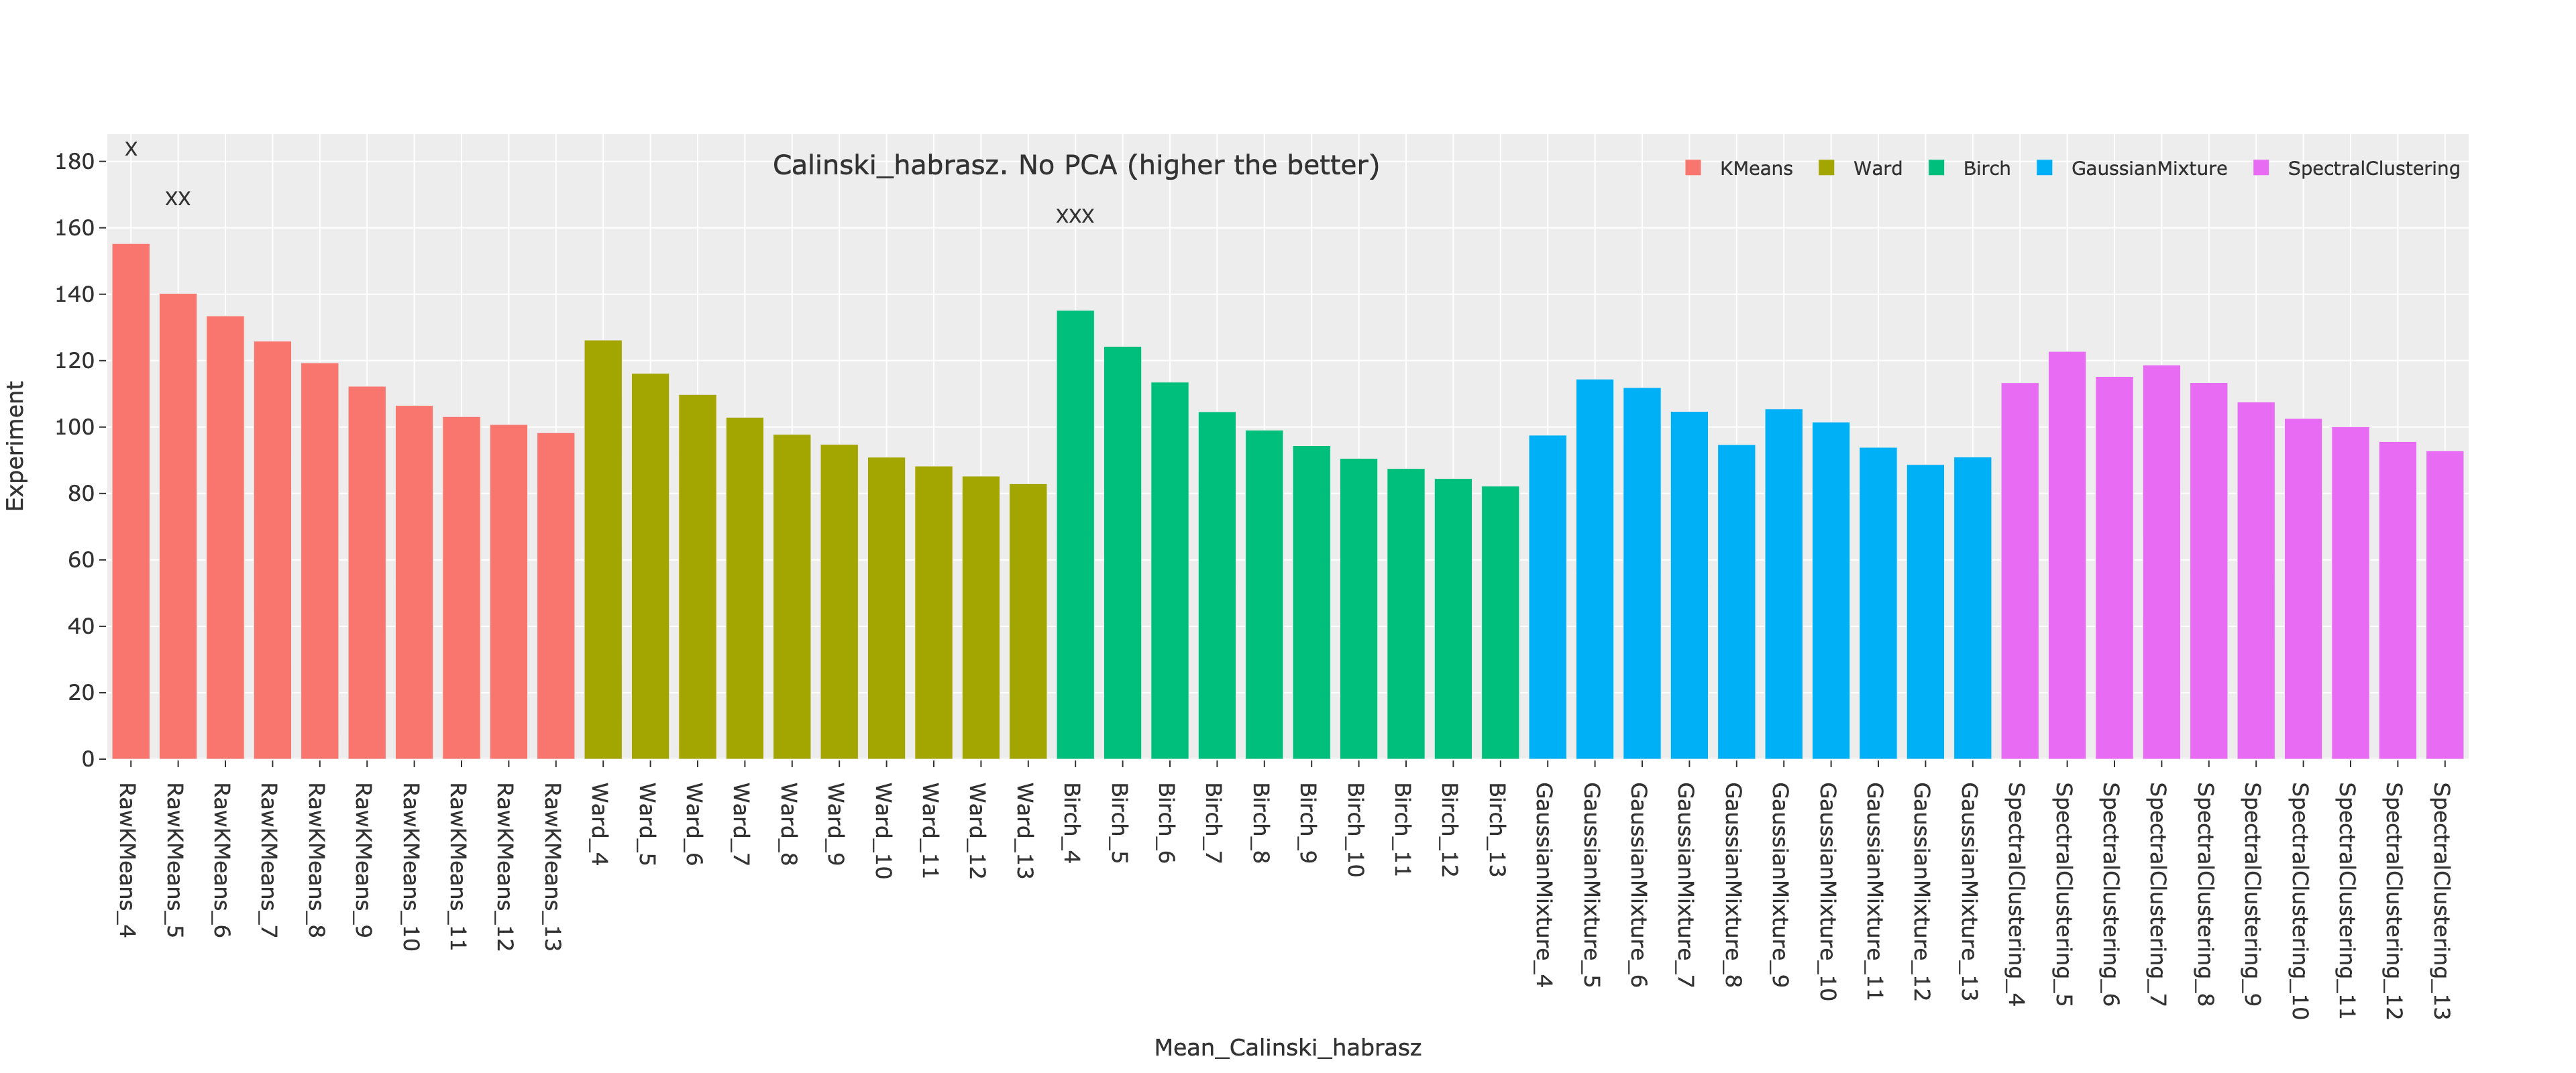
\includegraphics[width=\textwidth,keepaspectratio]{Sections/ClusteringAnalysis/Resources/cs_top3/PCA_top3_Calinski_habrasz.png}
        \caption{Calinski Harabasz}
        \label{fig:ap:cal_hab}
    \end{subfigure}
    \caption[Non-PCA transformed data: Silhouette and Calinski-Harabasz]{The means of the three cluster metrics introduced in \cref{s:lit:clustering_metrics}: Silhouette (cosine) and Calinski-Harabasz. For each metric, the top 3 performing models are marked by "X". Gaussian Mixture Model is abbreviated as GM, and Spectral Clustering as SC. K-means with K=4 and K=5 are the best-performing clustering configurations. The difference between this plot and the one in \cref{fig:cs:cs_metrics} is that the gene expression data here is not PCA-transformed. Overall, the non-PCA experiments perform worse compared to the PCA-transformed data in the two presented metrics and in the Davies-Bouldin score shown in \cref{fig:ap:non_pca_dav_boul}.}
    \label{fig:ap:non_pca_metrics}
\end{figure}

% Table of genes used in the Pi-plot
\section{Marker genes for Pi plot} \label{s:ap:pi_genes} 


\begin{table}[H]
    \centering
    \scriptsize
    \begin{tabularx}{\textwidth}{>{\hsize=0.6\hsize}X|>{\hsize=1.4\hsize}X|>{\hsize=1\hsize}X}
        \toprule
        \textbf{Name} & \textbf{Genes} & \textbf{Notes/Reference} \\
        \midrule
        \textbf{Luminal Markers} & KRT20, PPARG, FOXA1, GATA3, SNX31, UPK1A, UPK2, FGFR3 & TCGA \cite{Robertson2017-mg} \\
        \midrule
        \textbf{Basal Markers} & CD44, KRT6A, KRT5, KRT14, COL17A1 & TCGA \cite{Robertson2017-mg} \\
        \midrule
        \textbf{Squamous Markers} & DSC3, GSDMC, TCGM1, PI3, TP53 & TCGA \cite{Robertson2017-mg} \\
        \midrule
        \textbf{Neural Differentiation} & MSI1, PLEKHG4B, GNG4, PEG10, RND2, APLP1, SOX2, TUBB2B & TCGA \cite{Robertson2017-mg} \\
        \midrule
        \textbf{Lund MES} & TP53, RB1, FGFR3, ANKHD1, VIM, ZEB2 & Lund \cite{Marzouka2018-ge} \\
        \midrule
        \textbf{KRT} & KRT13, KRT14, KRT15, KRT20 & Family of genes - Lund \cite{Marzouka2018-ge}\\
        \midrule
        \textbf{UPK} & UPK1B, UPK1A, UPK3A, UPK2 & Family of genes - Lund \cite{Marzouka2018-ge}\\
        \midrule
        \textbf{CLD} & CLDN3, CLDN4, CLDN5 & Urothelial tight junction \cite{Smith2015-rj}  \\
        \midrule
        \textbf{serp} & SERPINB13, SERPINB3, SERPINB4 & Specific to Basal groups (Empirical observations) \\
        \midrule
        \textbf{spr} & SPRR1A, SPRR1B, SPRR2A, SPRR2D, SPRR3 & Specific to Basal groups (Empirical observations) \\
        \midrule
        \textbf{FGFR Family} & FGFR1, FGFR2, FGFR3, FGF1, FGF2 & Family of genes - differentiation \\
        \midrule
        \textbf{PI3K Pathway} & PIK3C3, PIK3R2, PIK3C2B, AKT1, AKT2 & Cell proliferation \citet{Sathe2018-cq} \\
        \midrule
        \textbf{sb\_ifng} & INFG, B2M, BATF2, BTN3A3, CD74, CIITA, CXCL10, CXCL9, EPSTI1, GBP1, GBP4, GBP5, HAPLN3, HLA-DPA1, IDO1, IFI30, IFI35, IFIT3, IFITM1, IL32, IRF1, NLRC5, PARP9, PSMB8-AS1, PSMB9, SAMHD1, SECTM1, STAT1, TAP1, TNFSF13B, TYMP, UBE2L6, WARS1, ZBP1 & \acrfull{ifn} gene signature \citep{Baker2022-bj} \\
        \midrule
        \textbf{Up Reg SCC} & BCL11B, BHLHE40, BNC1, EGR1, FOSL1, HES2, HMGA2, HOXD11, IRX3, JUN, KLF10, KLF13, KLF16, KLF4, MAFB, MYC, NFIL3, PITX1, SNAI2, SOX15, SOX7, TEAD4, TFAP2A, TIGD1, TRPS1, TWIST1, ZFPM2, ZNF598 & Up-regulated in \acrfull{scc} \citep{Hurst2022-sp} \\
        \bottomrule
    \end{tabularx}
    \caption[Gene markers used in pi-plots - part 1]{Gene markers used across the different Pi and Volcano plots to highlight different functions (Part 1). These were shown across various plots in the new MIBC found using the cluster analysis in \cref{s:cs:bio_interp} and the groups derived from the network approach in \cref{s:N_II:dea_rwd}. }
    \label{tab:ap:pi_genes_1}
\end{table}


\begin{table}[H]
    \centering
    \scriptsize
    \begin{tabularx}{\textwidth}{>{\hsize=0.6\hsize}X|>{\hsize=1.6\hsize}X|>{\hsize=.8\hsize}X}
        \toprule
        \textbf{Name} & \textbf{Genes} & \textbf{Notes/Reference} \\
        \midrule
        \textbf{Down Reg SCC} & BHLHE41, ELF3, FOXA1, FOXQ1, GATA3, HNF1B, HOXA13, IKZF2, IKZF3, IRF2, MECOM, PATZ1, POGK, PPARG, REPIN1, TBX2, TBX3, THYN1, TIGD2, ZFP14, ZFP30, ZFP62, ZNF100, ZNF124, ZNF132, ZNF136, ZNF14, ZNF181, ZNF195, ZNF20, ZNF222, ZNF223, ZNF230, ZNF233, ZNF248, ZNF253, ZNF254, ZNF257, ZNF273, ZNF28, ZNF320, ZNF41, ZNF420, ZNF429, ZNF43, ZNF430, ZNF439, ZNF440, ZNF443, ZNF461, ZNF486, ZNF492, ZNF493, ZNF506, ZNF518A, ZNF528, ZNF546, ZNF563, ZNF568, ZNF585A, ZNF585B, ZNF615, ZNF620, ZNF625, ZNF627, ZNF675, ZNF678, ZNF680, ZNF682, ZNF69, ZNF708, ZNF709, ZNF714, ZNF717, ZNF726, ZNF730, ZNF735, ZNF737, ZNF763, ZNF780B, ZNF792, ZNF793, ZNF799, ZNF844, ZNF85, ZNF90, ZNF91, ZNF92, ZNF93, ZNF98, ZSCAN16 & Down-regulated in \acrfull{scc} \cite{Hurst2022-sp} \\
        \midrule
        \textbf{Macrophages} & ADGRE1, CCR2, CD14, CD68, CSF1R, Ly6c1, MARCO, MRC1, NOS2, SIGLEC1, TLR2, ARG1, CD163, CD200R1, CD80, CD86, CLEC10A, CLEC7A, CSF2, CX3CR1, FCGR1A, ITGAM, MERTK, PDCD1LG2, TNF, CCL22, CD36, CD40, IL10, IL1B, IL6, LGALS3, TLR4, CCL2, CCR5, CD209, CD63, CD86, CSF1, CXCL2, FCGR3A, ITGAX, MSR1, PTPRC, STAT6, TIMD4, Chil3, CLEC6A, IL1R1, ITGB2, PDCD1LG2, TLR7 & Immune specific, empirically observed across the \acrlong{dea} experiments from \cref{s:cs:basal_interp} \\
        \midrule
        \textbf{Monocytes} & CD14, CD16, CSF1R, CX3CR1, ITGAM, ITGAX, LY6C1, CCR2, CXCR4, FCGR1A, SELL, SPN, ADGRE1, CCR7, TNF, CD86, IL10, IL1B, MERTK, TREML4, CD209, NR4A1, Ly6a, PTPRC, IL3RA, CD27, CCR5, CD32, CD1A, MRC1, ITGB3, CD9, CXCR6, CCR1, FLT3, KLF2, CLEC12A, CCR6, CCR8, CD68, CLEC7A, KIT, MAF, MAFB, SPI1, CD1C, PPARG, CEBPB, ITGAE, TEK &  Immune specific, empirically observed across the \acrlong{dea} experiments from \cref{s:cs:basal_interp} \\
        \midrule
        \textbf{B Cells} & BCL2, BCL6, CD19, CD1D, CD22, CD24, CD27, CD274, CD34, CD38, CD40, CD44, CD5, CD53, CD69, CD72, CD79A, CD79B, CD80, CD86, CD93, CR2, CXCR4, CXCR5, FAS, FCER2, FCRL4, HAVCR1, IL10, IL2RA, IL7R, IRF4, ITGAX, LILRB1, MME, MS4A1, NT5E, PDCD1LG2, PRDM1, PTPRC, SDC1, SPN, TFRC, TLR9, TNFRSF13B, TNFRSF13C, TNFRSF17, XBP1 & Immune specific, empirically observed across the \acrlong{dea} experiments from \cref{s:cs:basal_interp} \\
        \midrule
        \textbf{ig\_fam} & IGHG1, IGHG3, IGHJ2, IGHJ3, IGHJ4, IGHM, IGHV1-69D, IGHV2-70, IGHV3-11, IGHV3-15, IGHV4-39, IGKC, IGKJ1, IGKJ4, IGKV1-5, IGKV1-6, IGKV1-9, IGKV1D-39, IGKV2-28, IGKV4-1, IGLC1, IGLC2, IGLC3, IGLJ2, IGLJ3, IGLV1-40, IGLV1-44, IGLV3-19 & Immunoglobulin family, empirically observed across the \acrlong{dea} experiments from \cref{s:cs:basal_interp} \\
        \bottomrule
    \end{tabularx}
    \caption[Gene markers used in pi-plots - part 2]{Gene markers used across the different Pi and Volcano plots to highlight different functions (Part 2). These were shown across various plots in the new MIBC found using the cluster analysis in \cref{s:cs:bio_interp} and the groups derived from the network approach in \cref{s:N_II:dea_rwd}.}
    \label{tab:ap:pi_genes_2}
\end{table}


% GSEA
\section{GSEA - Hallmarks for NE} \label{s:ap:cs:gsea_ne}

\begin{figure}[H]    
    \centering
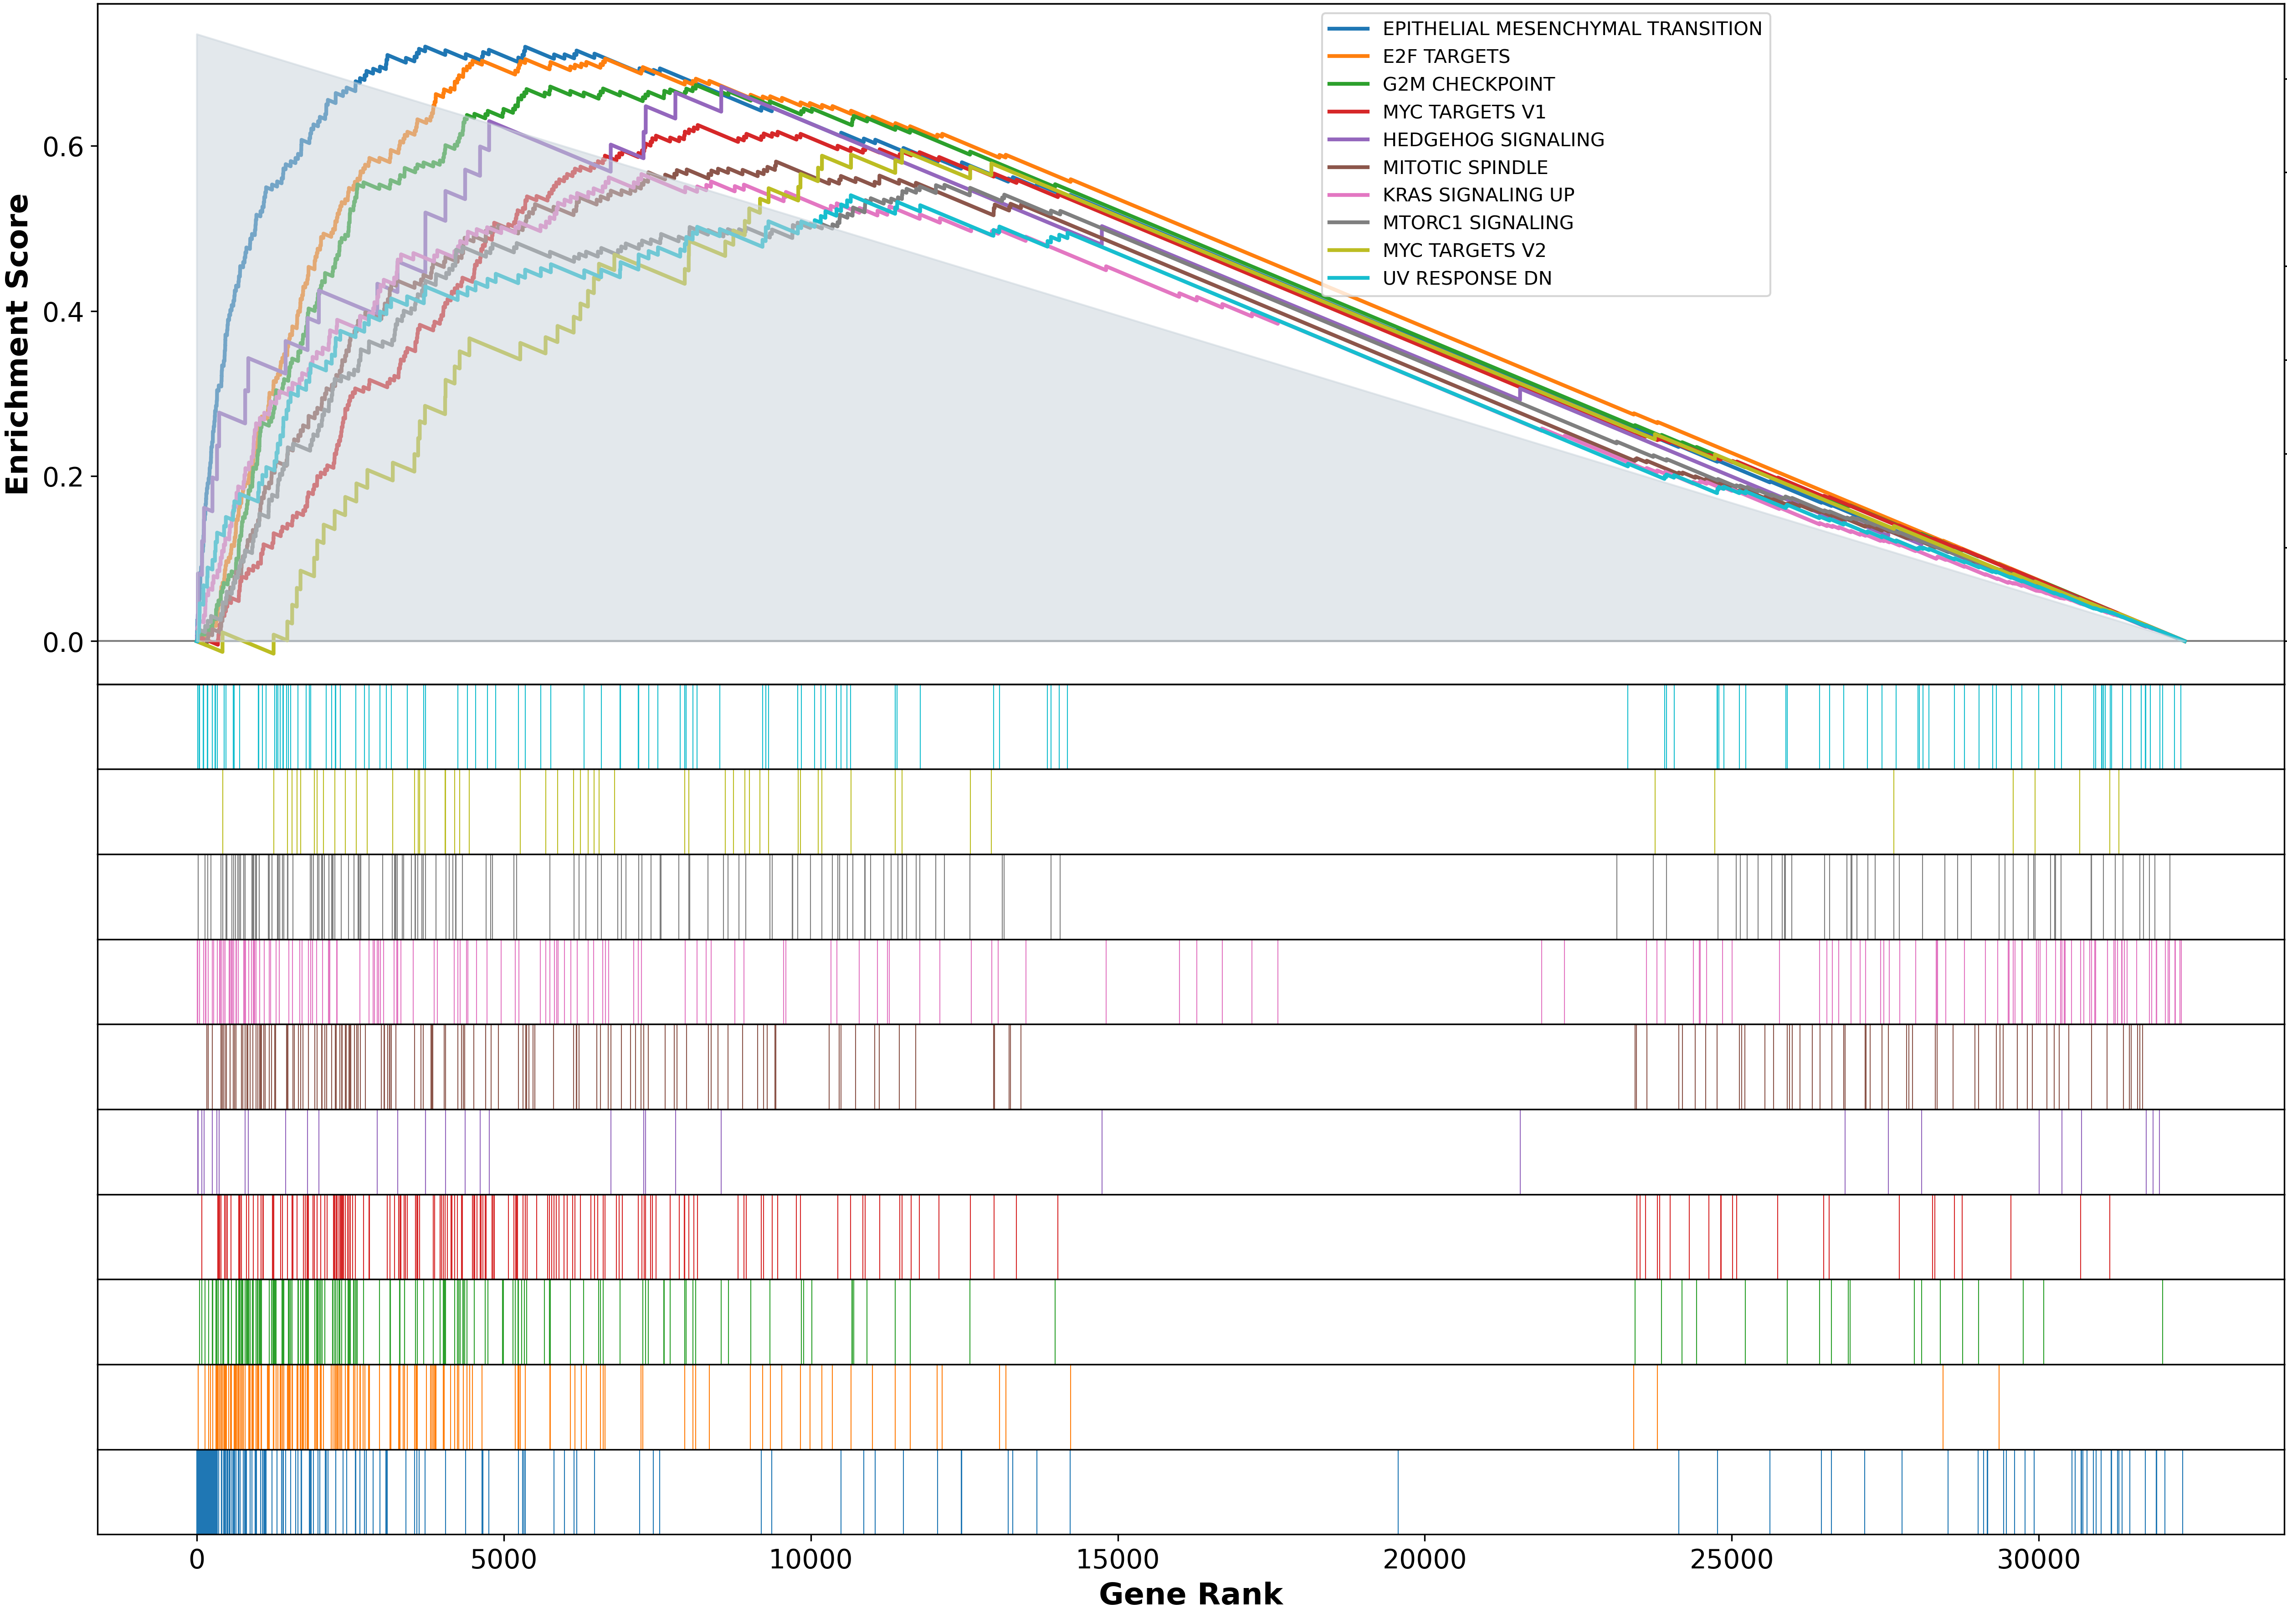
\includegraphics[width=1.0\textwidth,keepaspectratio]{Sections/ClusteringAnalysis/Resources/discussion/other_groups/ne2_hallmark_10_top.png}
     \caption[GSEA markers for Ne-like group]{For the Neuroendocrine-like group derived in \cref{s:cs:bio_interp} and accompanying the analysis in \cref{s:cs:ne_interp}. The top 10 terms of running GSEA on the Hallmark database. The gene ranking for GSEA is using distance from the 'Ref point' in \cref{fig:cs:ne_pi} to all the other genes. The closest points to the 'Ref point' also have the highest ranking for GSEA. The results show that there pathways involved in cell-cycle for the closest genes to the 'Ref point'. See \cref{fig:cs:ne_gsea} for the GSEA results when using the Reactome database. }
    \label{fig:ap:cs:gsea_ne_hallmark}
\end{figure}


% \subsection{LumInf}

% \begin{figure}[H]    
%     \centering
% 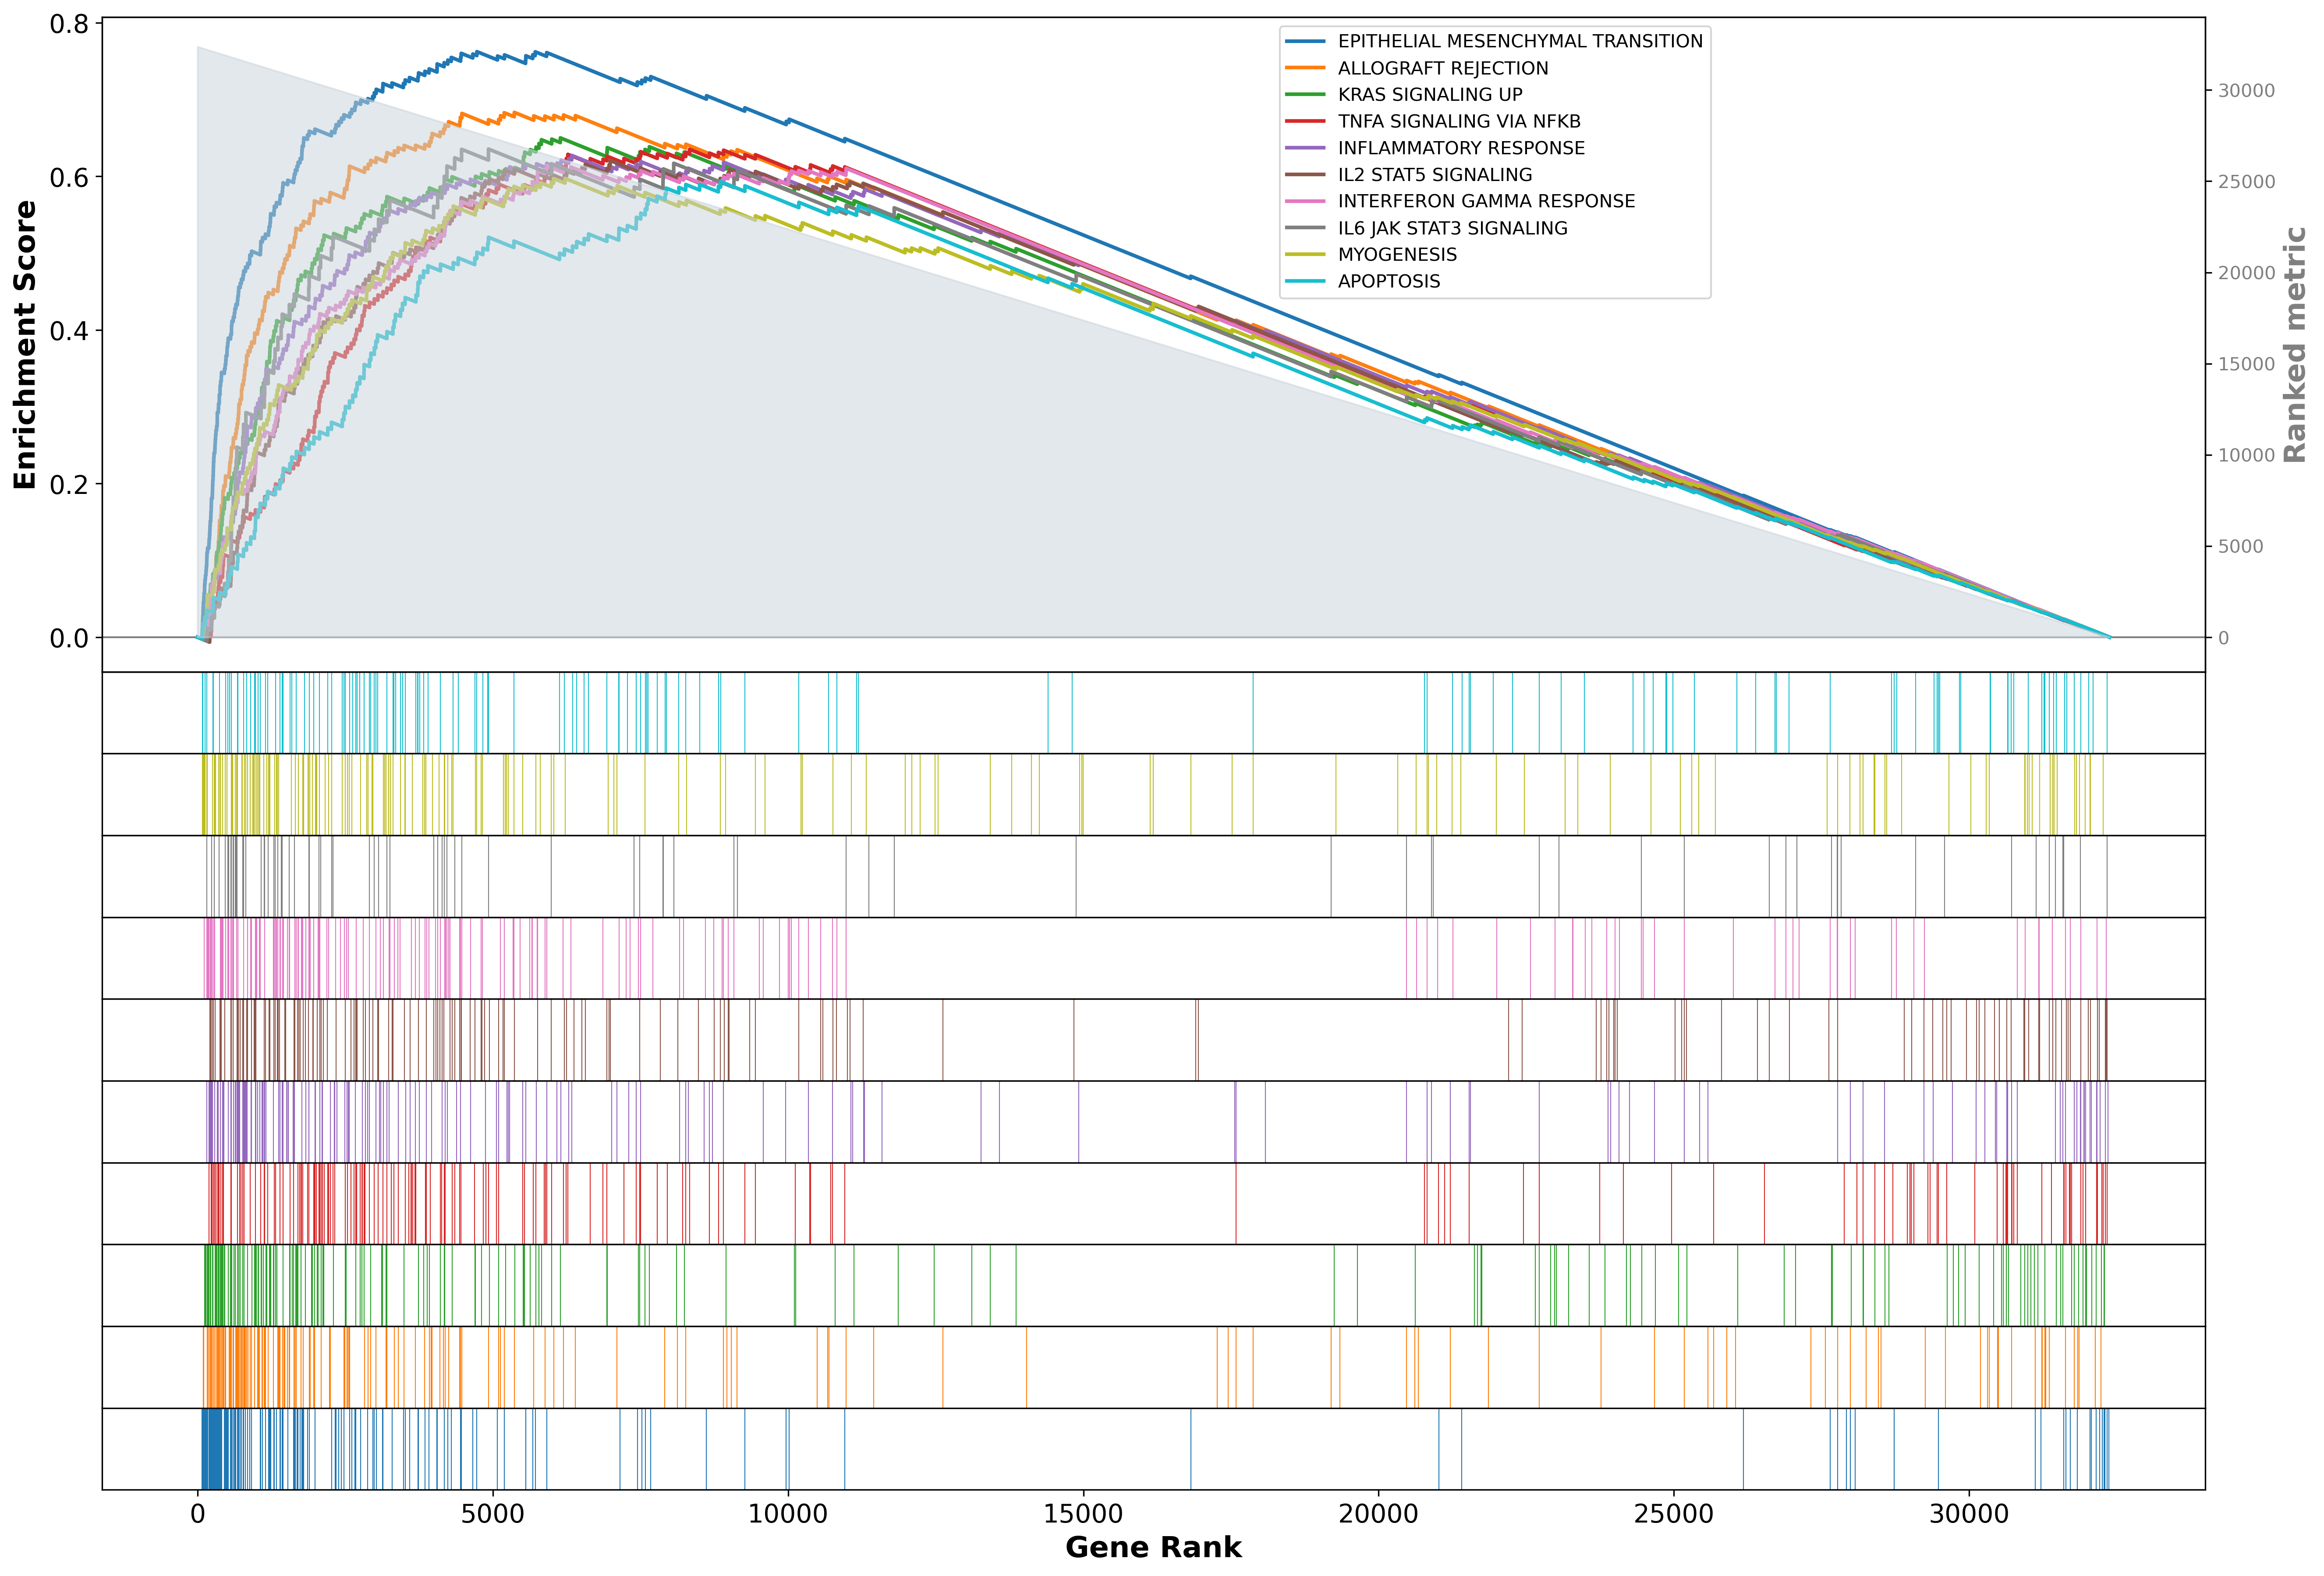
\includegraphics[width=1.0\textwidth,keepaspectratio]{Sections/ClusteringAnalysis/Resources/discussion/other_groups/lumInf_hallmark_10_top.png}
%     \caption{For the Luminal Infiltrated group derived in \cref{s:cs:bio_interp} and accompanying the analysis in \cref{s:cs:lumInf_interp}. The top 10 terms of running GSEA on the Hallmark database. The ranking is using the pi plot from \cref{fig:cs:lumInf_pi}}
%     \label{fig:ap:cs:gsea_lumInf_hallmark}
% \end{figure}


% \subsection{LumP}


% \begin{figure}[H]    
%     \centering
% 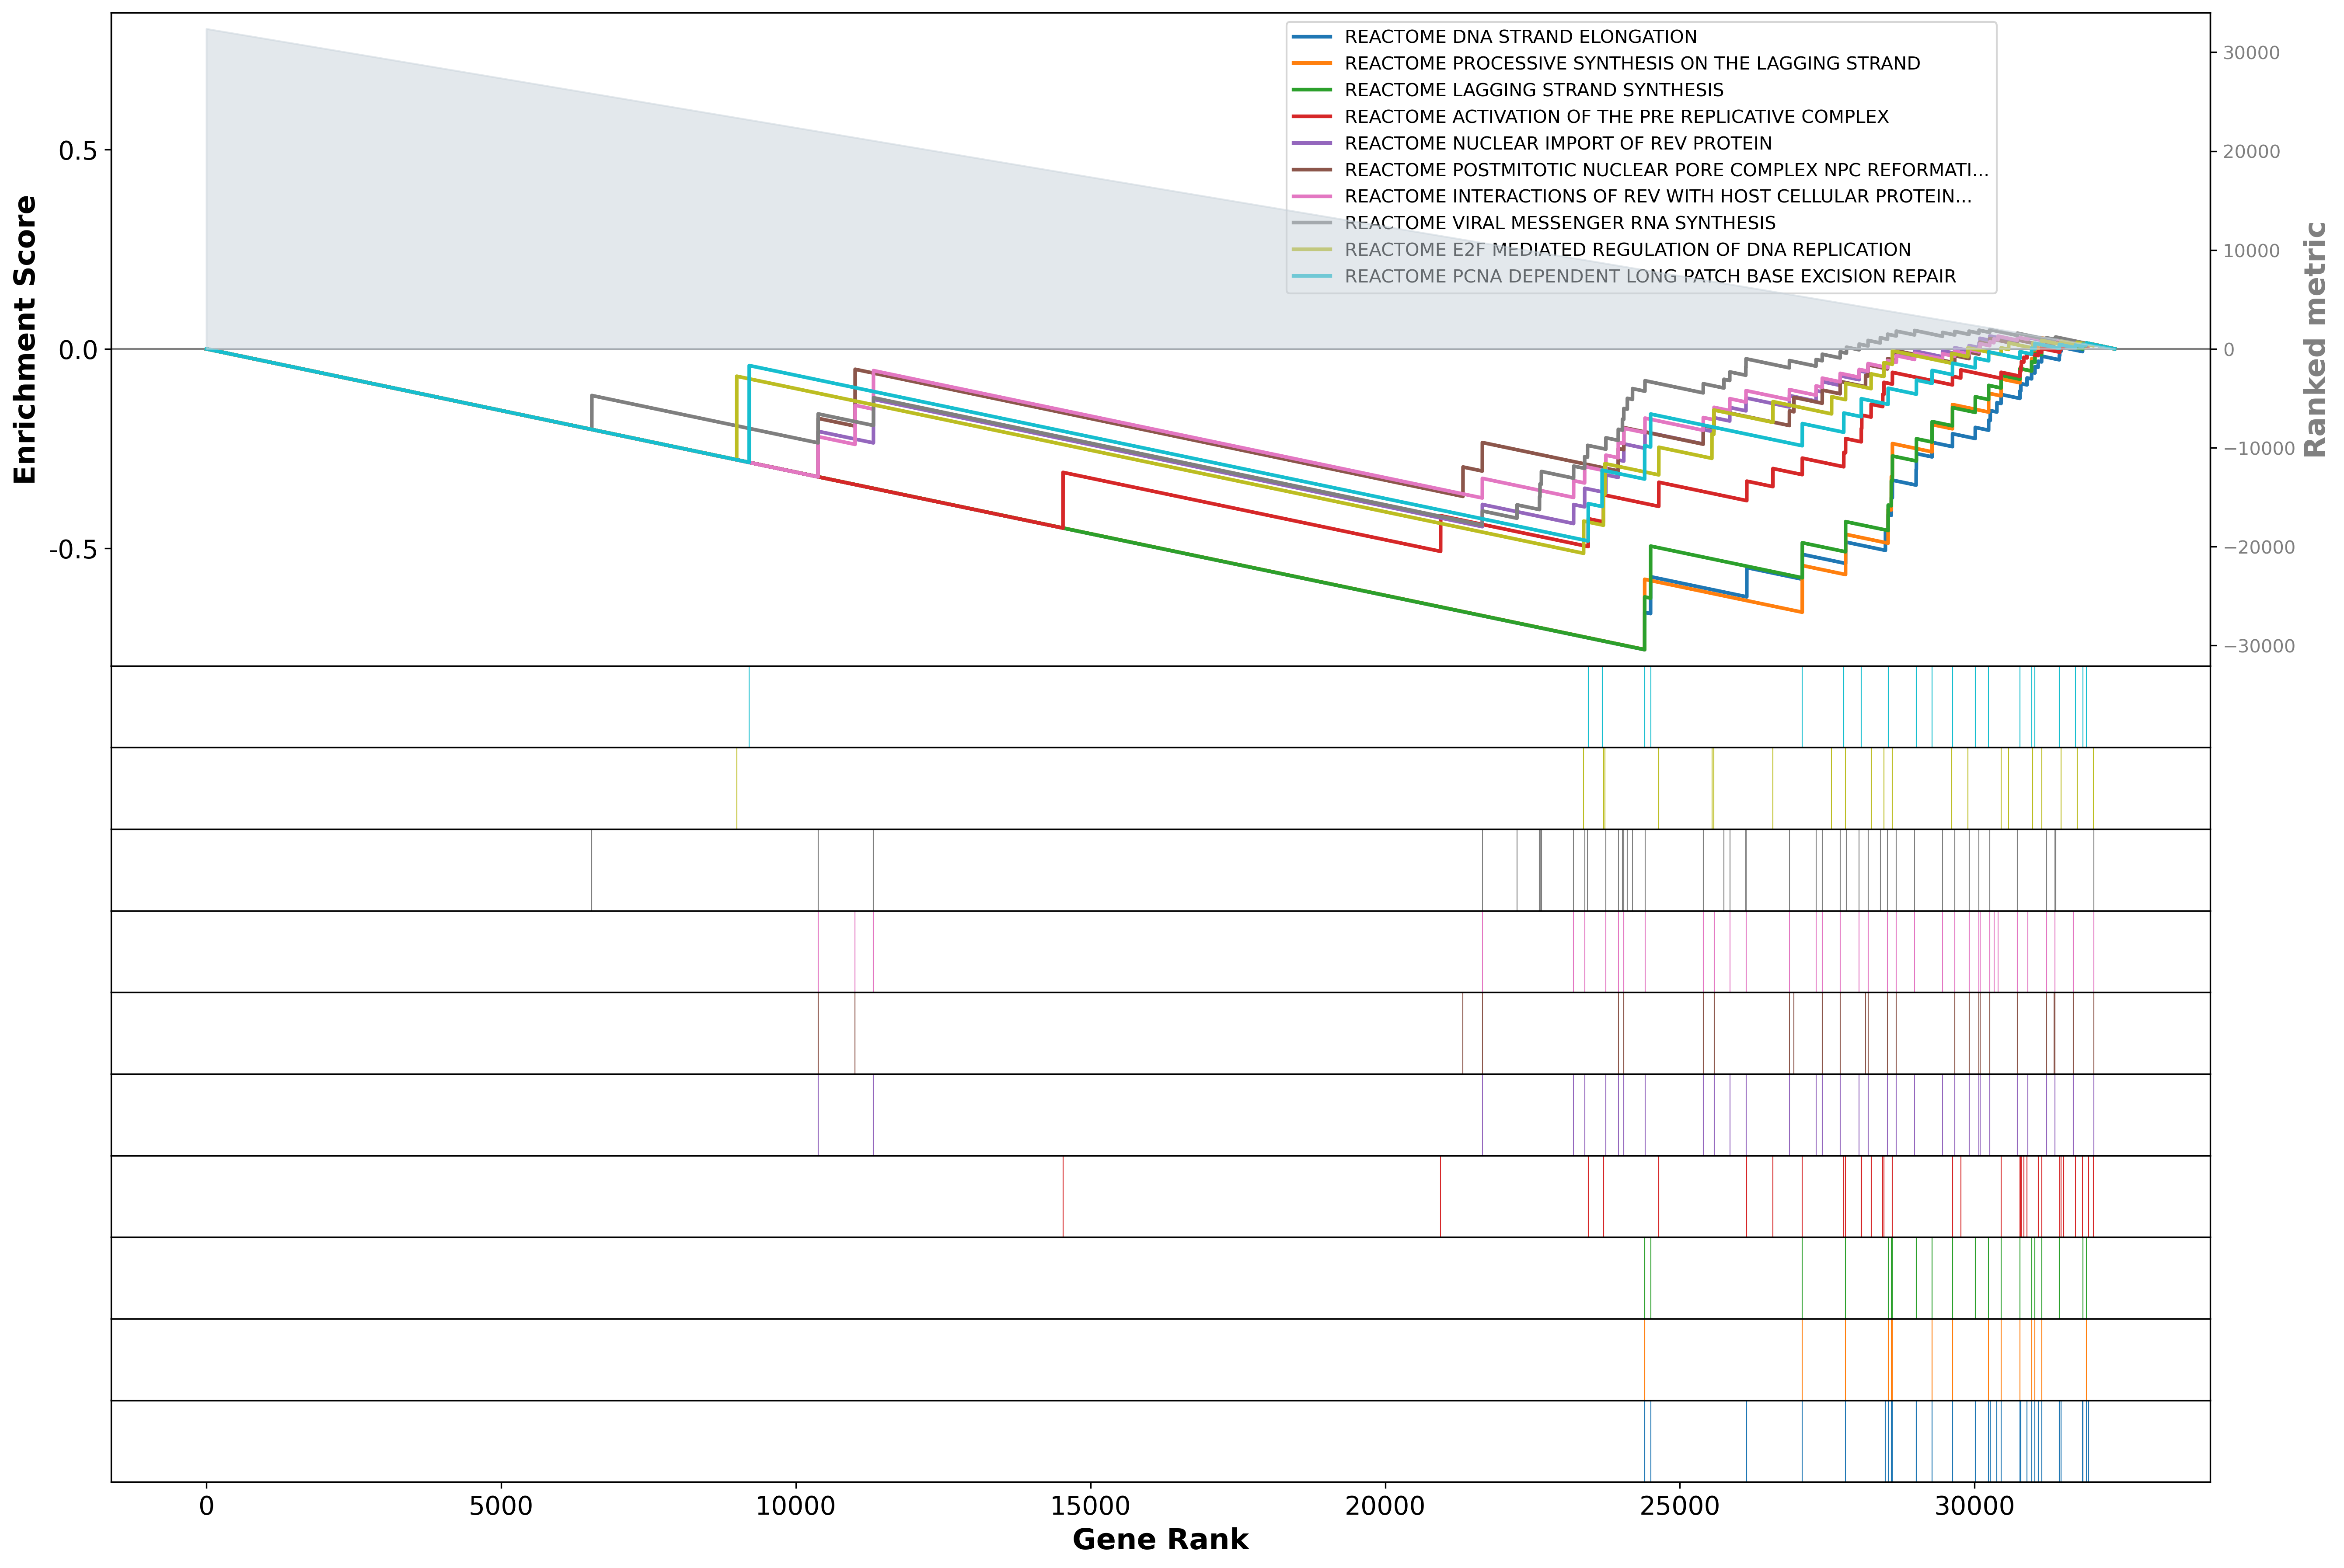
\includegraphics[width=1.0\textwidth,keepaspectratio]{Sections/ClusteringAnalysis/Resources/discussion/other_groups/lumP2_hallmark_10_top.png}
%      \caption{For the Luminal Papillary group derived in \cref{s:cs:bio_interp} and accompanying the analysis in \cref{s:cs:lumP_interp}. The top 10 terms of running GSEA on the Hallmark database. The ranking is using the pi plot from \cref{fig:cs:lumP_pi}}
%     \label{fig:ap:cs:gsea_lump_hallmark}
% \end{figure}
